% thesis.tex
%
% requirements
%   jsclasses
%   thesis.sty
%

%% JISフォントメトリックが用意されていない場合(debian等)は,
%% 従来のmingothを用いる.
%\documentclass[mingoth,11pt,openany,a4paper]{jsbook}
%% 標準
%% openanyを省くと,右側のページから章がはじまる
	
% pdf用の文書情報
\input docinfo.out

\documentclass[12pt,a4paper]{jsbook}

\usepackage{graphicx}

\usepackage{bm}
\usepackage{amscd}
\usepackage{amssymb}
\usepackage{amsfonts}
\usepackage{multicol}
\usepackage{amsmath}
\usepackage{array}
\usepackage{subfigure}

\graphicspath{{./figures/}}

% TXフォントを使う
\usepackage{txfonts}

% 独自論文スタイルの使用
\usepackage{thesis}

% for dvipdfm
\usepackage[dvipdfmx]{color}
%\usepackage[dvipdfmx,bookmarks=true,bookmarksnumbered=true,bookmarkstype=toc,%
%    pdftitle=\PDFTITLE, %
%    pdfsubject=\PDFSUBJECT, %
%    pdfauthor=\PDFAUTHOR, %
%    pdfkeywords=\PDFKEYWORDS]{hyperref}
%\ifnum 42146=\euc"A4 \AtBeginDvi{\special{pdf:tounicode EUC-UCS2}}\else
%\AtBeginDvi{\special{pdf:tounicode 90ms-RKSJ-UCS2}}\fi

% 一行の文字制限(40zw)をなくす
\setlength{\textwidth}{\fullwidth}
\renewcommand{\baselinestretch}{1.1}
\setcounter{tocdepth}{2}

% evensidemarginの再定義
% この部分は jsbook.cls の定義と同じです.
% jsbook.cls の定義がかわっていれば,そちらにあわせて下さい.
\setlength{\evensidemargin}{\oddsidemargin}
\addtolength{\evensidemargin}{\fullwidth}
\addtolength{\evensidemargin}{-\textwidth}

% とじしろの確保
% defaultではとじしろがないので,その分ずらします.
\addtolength{\oddsidemargin}{8mm}
\addtolength{\evensidemargin}{-8mm}

% \renewcommand{\baselinestretch}{1.38}
% \kanjiskip=.1zw plus 3pt minus 3pt
% \xkanjiskip=.1zw plus 3pt minus 3pt

% \makeatletter
% \renewcommand{\theequation}{\thesection.\arabic{equation}}
% \@addtoreset{equation}{section}

% \renewcommand{\thetable}{\thesection.\arabic{table}}
% \@addtoreset{table}{section}

% \renewcommand{\thefigure}{\thesection.\arabic{figure}}
% \@addtoreset{figure}{section}

% \renewcommand{\paragraph}{\@startsection{paragraph}{4}{\z@}%
%    {1.5\Cvs \@plus.5\Cdp \@minus.2\Cdp}%
%    {.5\Cvs \@plus.3\Cdp}%
%    {\reset@font\normalsize\bfseries}}
%    
% \makeatother

\DeclareMathOperator{\sgn}{sgn}

\frontmatter

% thesis(論文の区別),title(題),date(提出日),teacher(指導教官),
% organization(所属), author(著者), \idnumber(学生証番号)

\thesis{修士学位論文} 
\title{表面構造を考慮した\\複眼のリアルタイムレンダリング}
% \engtitle{Detailed Surface Representation of Fluid by Multi-scale Simulation}
\organization{東京大学大学院 学際情報学府}
\course{先端表現情報学コース} %%所属
\date{平成26年度}
\author{佐川 和輝}
\teacher{河口 洋一郎 教授}
\idnumber{136313}

\begin{document}

% 表紙
\maketitle

%\include{abstract}

% 目次
\thispagestyle{headings}
\tableofcontents

% 図一覧
\thispagestyle{headings}
\listoffigures

%表一覧
\thispagestyle{headings}
\listoftables

\mainmatter

\chapter{*タイトル*}
\label{*Ltitle*}

タイトルの中身だよ。

\subsection{サブセクション}
\label{*Lsubsection*}

サブセクション\cite{*AuthorName*}の中身だよ。\figref{test} %画像番号。(Fig1.1)など



\begin{itemize}
\item アイテム1
\item アイテム2
\item アイテム3。文章に出来るよ
\end{itemize}

\begin{figure}[h]
  \centering
  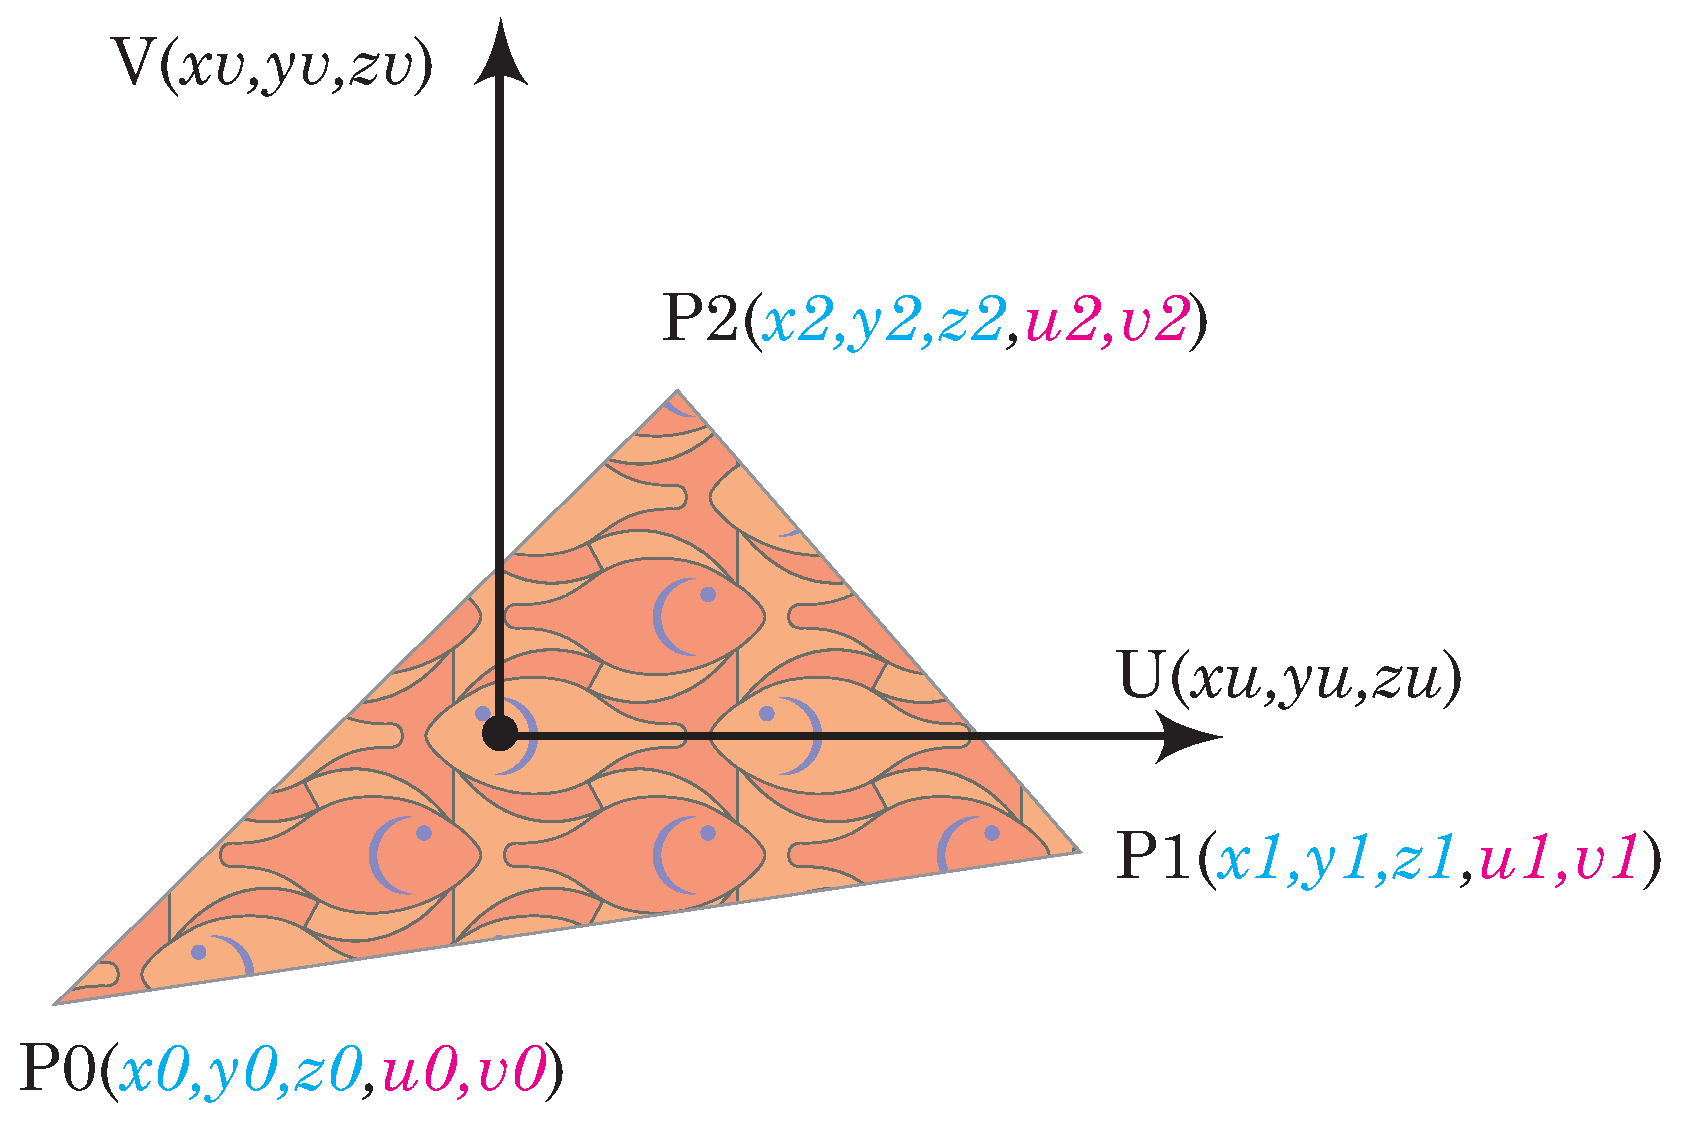
\includegraphics[width=3.0in]{./img/polygon_explain}
  \caption{キャプションだよ}{行を変えられるみたい}
  \label{test} %ここで画像のラベリング?
\end{figure}
 
        %テンプレート
\chapter{序論}
\label{CBegin}

\section{*研究背景*}
\label{SBackground}

ばっくぐらうんどー
	%1章 序論
\chapter{関連研究}
\label{CRelatedWork}

りれーてっどわーく。
	%2章 関連研究
\chapter{周辺技術}
\label{CTechnology}

本章では、……と関連の深いなんとかかんとか。
	%3章 周辺技術
\chapter{提案手法}
\label{CMethod}

\secref{SBackground}セクションリファレンス
とらとらとら。
		%4章 提案手法
\chapter{予備実験}
\label{CExperiment}

\section{実験の目的}
\label{SExperimentPurpose}

実験の目的は……これこれこういうことですよ~。

\section{実験方法}
\label{SExperimentMethod}

こんな風にして実験を行いましたよん。
	%5章 シミュレーション実験
\chapter{結果と考察}
\label{CResult}

\section{*サブセクション*}
\label{SSubsection}

さぶせく~~。
		%6章 結果と考察
\chapter{結論}
\label{CConclusion}

\section{結論}
\label{SConclusion}

本研究では、複眼のリアルタイムレンダリングを行った。などなど。
以下の成果を確認できた。

\begin{itemize}
\item 
\item 
\item 
\item 
\end{itemize}

本研究は~だけではなく…………。


\section{今後の展望}
\label{SFutureWork}

\chapref{SConclusion}で既述したように…………。といった使い方ができる。
	%7章 結論
\addcontentsline{toc}{chapter}{謝辞}
\chapter*{謝辞}

あとは謝辞をつらつらと書くだけよん♪
	%謝辞


%参考文献
\bibliographystyle{junsrt}
\bibliography{papers_bib}

% 付録
%\appendix
%\include{appendix}

\clearpage

\backtitle

\end{document}
